\chapter{Grundlagen von Data Analytics}
\bauer
	
	\section{Data Analytics}
	
		%Quellen: https://en.wikipedia.org/wiki/Data_analysis
		\subsection{Definition} \footcite{data-analysis}
			Data Analytics ist ein Prozess bei dem Daten inspiziert, gereinigt, verwandelt und modelliert werden um neue nützliche Informationen zu bekommen. Dies Dient vor allem als Hilfestellung bei wichtigen Entscheidungen. Eines der Ziele von Data Analytics ist es Firmen dabei zu unterstützen effizienter zu arbeiten. 
	
		\subsection{Vorgehensweise}
		
			\subsubsection{Anforderungen}
				Zuerst muss festgelegt werden welche Daten analysiert werden, woher diese Daten kommen und wie die Daten aufgebaut sind. Dies hängt meistens von dem Zweck der Datenanalyse ab. Ein weiter Punkt welcher beachtet werden muss ist das Ergebnis welches erwartet wird von der Analyse.
			
			\subsubsection{Sammlung}
				Die Sammlung der Daten kann von verschiedenen Quellen stattfinden sowohl firmenintern als auch externe Quellen wie das Internet oder externe Datenbanken. Bevor mit der Analyse begonnen werden kann müssen die Quellen erkannt und strukturiert werden. Die Datenmenge muss in diesem Schritt ebenfalls in Betracht gezogen werden. Wenn sich um eine geringe Datenmenge haltet kann die Analyse meist auf einem der Server statt finden welche normalerweise für andere Prozesse verwendet werden. Eventuell reicht bei sehr kleinen Datenmengen auch der Standrechner von den Personen welche die Analyse durchführen. Bei sehr großen Mengen kann es passieren, dass für den Prozess ein extra Server gekauft oder gemietet werden muss. 
			
			\subsubsection{Verarbeitung}
				Bei der Verarbeitung werden die verschiedenen Datenquellen in eine Struktur gebracht welche alle für die spätere Verwendung benötigt wird diese unterscheidet sich je nach Anwendungsfall. Bei diesem Prozess muss darauf geachtet werden das keine der wichtigen Informationen verloren gehen. 
			
			\subsubsection{Reinigung}
				Während der Reinigung werden redundante so wie nicht benötigte Informationen gelöscht dies reduziert die Datenmengen was für besser Performance und einen geringeren Speicherverbrauch sorgt. Dies ist besonders bei großen Datenmengen sehr wichtig. Bei der Reinigung können in vielen Fällen Muster oder auffällige Daten erkannt werden, welche oft einen Ausblick auf das zu erwartenden Ergebnis liefert. 
			
			\subsubsection{Erkundung}
				Durch die Erkundung werden bisher unbekannte Zusammenhänge in den unterschiedlichen Quellen erkannt. Dies kann durch verschiedene Verfahren erreicht werden. Eines der meist verwendeten Methoden ist die explorative Datenanalyse welche ein Teilgebiet der Statistik ist. Dieses Verfahren wird meistens von Diagrammen wie Box-Plot oder Mosaik-Plot unterstützt weiterhin gibt es verschiedene Softwares wie GeoDa oder MANET welches oft kostenlos sind. 
				 
			\subsubsection{Modellierung}
				In der Modellierung werden verschiedene Algorithmen auf die Daten angewendet dies dient vor allem dem Entdecken von Zusammenhänge welche durch die explorative Datenanalyse nicht erkannt werden konnte. 
			
			\subsubsection{Kommunikation}
				Während der Kommunikationsphase werden die Ergebnisse in verschiedenen Formen präsentiert meist unterstützt durch graphische Diagramme welches die effiziente Kommunikation unterstützen. Bei dieser Präsentation sollte daran gedacht werden, dass viele der Entscheidungsträger für welche die Information gedacht ist sich oft nicht mit technischen Spezifikationen aufhalten möchten. 
			
		% Quelle: https://hackr.io/blog/what-is-data-analysis-methods-techniques-tools
		\subsection{Analyse Methoden} \footcite{analyse-methode}
		
			\subsubsection{Qualitative Analyse}
				In der Qualitative Analyse werden die Fragen "wie?" "was?" und "warum?" indem quantitative Techniken angewendet werden  wie Fragebögen oder Einstellungsskalierungen. Diese Analyse kommt für gewöhnlich in Form von Text was eventuell auch durch Audio und Video unterstützt wird. 
				
			\subsubsection{Quantitative Analyse}
				Diese Form der Analyse ist mit Zahlen gestützt die Daten werden an klar definierten Werten festgelegt welches die Darstellung durch Graphen ermöglicht. 
				
			\subsubsection{Text Analyse}
				In dieser Art der Analyse wird Text analysiert um Fakten zu extrahieren welche von Maschinen verstanden werden können. Das Ziel darin liegt strukturierte Information aus unstrukturierten Inhalten zu erstellen. Diese Form der Analyse wird auch als "Text-Mining" bezeichnet.
			
			\subsubsection{Statistische Analyse}
				Bei der statistischen Analyse werden Datensammlungen, Interpretation und Validierungen verwendet um verschiedene statistische Operationen durchzuführen. Die meisten Daten die verwendet werden sind beschreibende Daten wie Fragebögen oder Beobachtungsdaten. 
			
			\subsubsection{Diagnostische Analyse}
				Die diagnostische Analyse ist eine Weiterführung der statistischen Analyse welche eine genauere Analyse ermöglicht. Diese Art der Analyse wird auch als Ursachenanalyse bezeichnet. Die Funktionsweise dieser Art von Analyse kann in drei Kategorien eingeteilt werden. \newline
				Anomalien identifizieren: In dieser Kategorie werden bestimmte Bereiche identifiziert welche genauere Analysen benötigen. \newline
				Bohr Analyse: In dieser Kategorien werden Datenquellen identifizierte dies hilft besonders beim erklären von Anomalien. Diese Form der Analyse benötigt oft Strukturen welche außerhalb der Daten liegen was bedeutet das externe Daten zur Analyse hinzugefügt werden müssen um alle Zusammenhänge zu erkennen.  \newline
				Klausel Zusammenhänge: In dieser Kategorien werden bisher unbekannte Zusammenhänge erkannt durch Wahrscheinlichkeitstheorie, Regressionsanalyse, Filterung und Zeitreihendatenanalyse wodurch versteckte Sachverhalte erkannt werden.  		
			
			\subsubsection{Vorausschauende Analyse}
				In der vorausschauende Analyse werden historische Daten in einen künstliche Intelligenz eingespielt um kritische Muster und Trends zu erkennen. Dieses Model wird danach auf die aktuellen Daten angewendet um zukünftige Trends zu erkennen. 
	
		\subsection{EMS Statistik}
			Die EMS-Software verwendet Data Analytik insbesondere in dem Interface der Administratoren da dieser einen Überblick über die gesamten Aktivitäten der User und über die Events benötigen.  
			
			\subsubsection{Verkaufte Karten}
				Bei dieser Statistik wird ein Balkendiagramm generiert welcher zeigt wie viele Karten pro Woche verkauft wurden. Wenn es verschieden Karten gibt werden diese in verschiedenen Farben pro Woche angezeigt. Diese Statistik hilft den Administratoren zu sehen wie viele Karten schon verkauft sind und abzuschätzen wie viel Erfolg das Event bietet. Durch diese Statistik kann auch ein Trend erkannt werden und gesehen werden wie gut bestimmte Werbemaßnahmen.
				
				\begin{figure}[H]
					\centering
					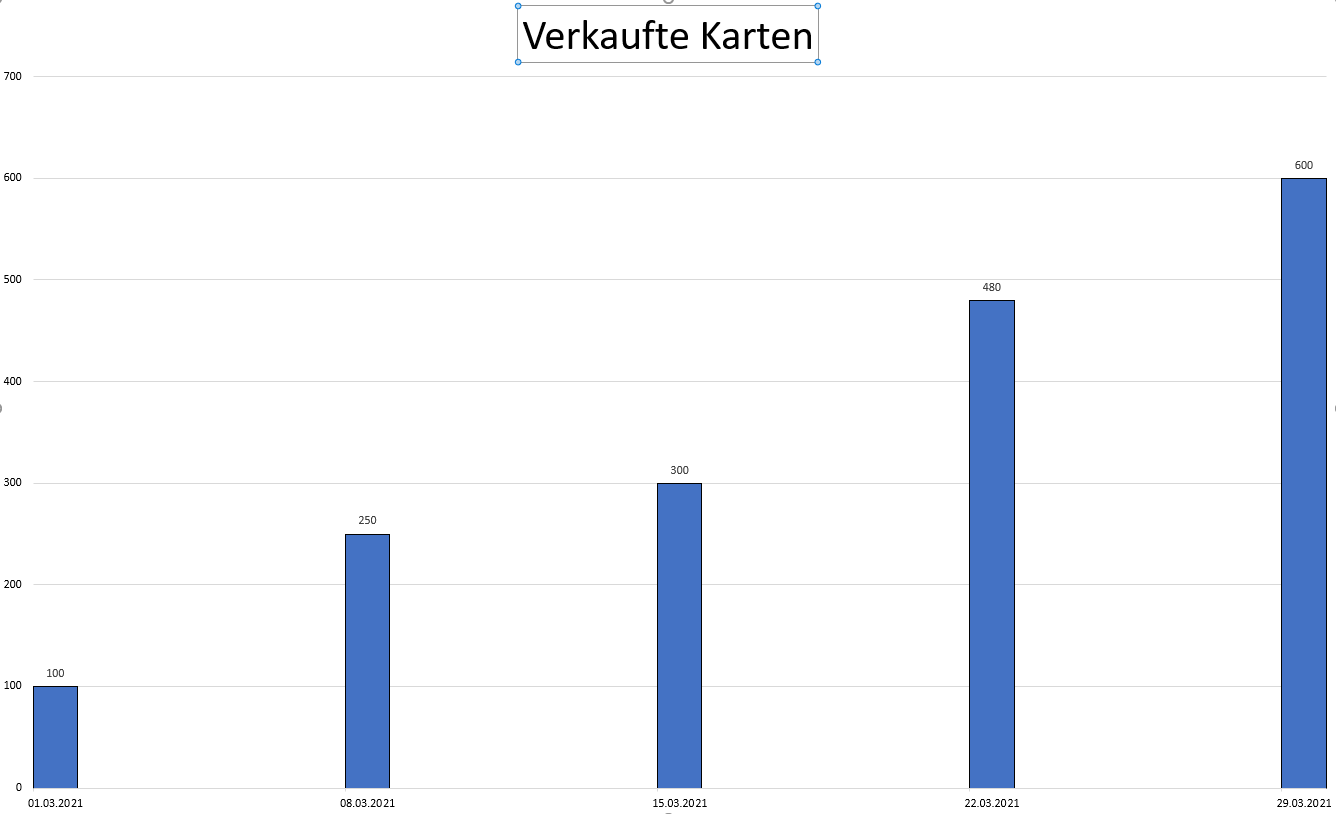
\includegraphics[width=\textwidth,height=\textwidth,keepaspectratio]{verkaufte_karten.PNG}
					\caption{Verkaufte Karten Diagram}
				\end{figure}

			\subsubsection{Verteilte Karten}
				Diese Statistik besteht aus einem Kreisdiagramm welches in 3 Kategorien aufgeteilt wird. Verkaufte Karten, Verteilte Karten, nicht verteilte Karten. Diese Statistik bietet einen simplen Überblick über die Kartenverteilung und es kann einfach erkannt werden ob mehr Promoter eingestellt werden müssen falls zu viele Karten noch nicht verteilt sind oder ob es zu wenig Karten gibt für die Anzahl an aktiven Promotern. 
				
				\begin{figure}[H]
					\centering
					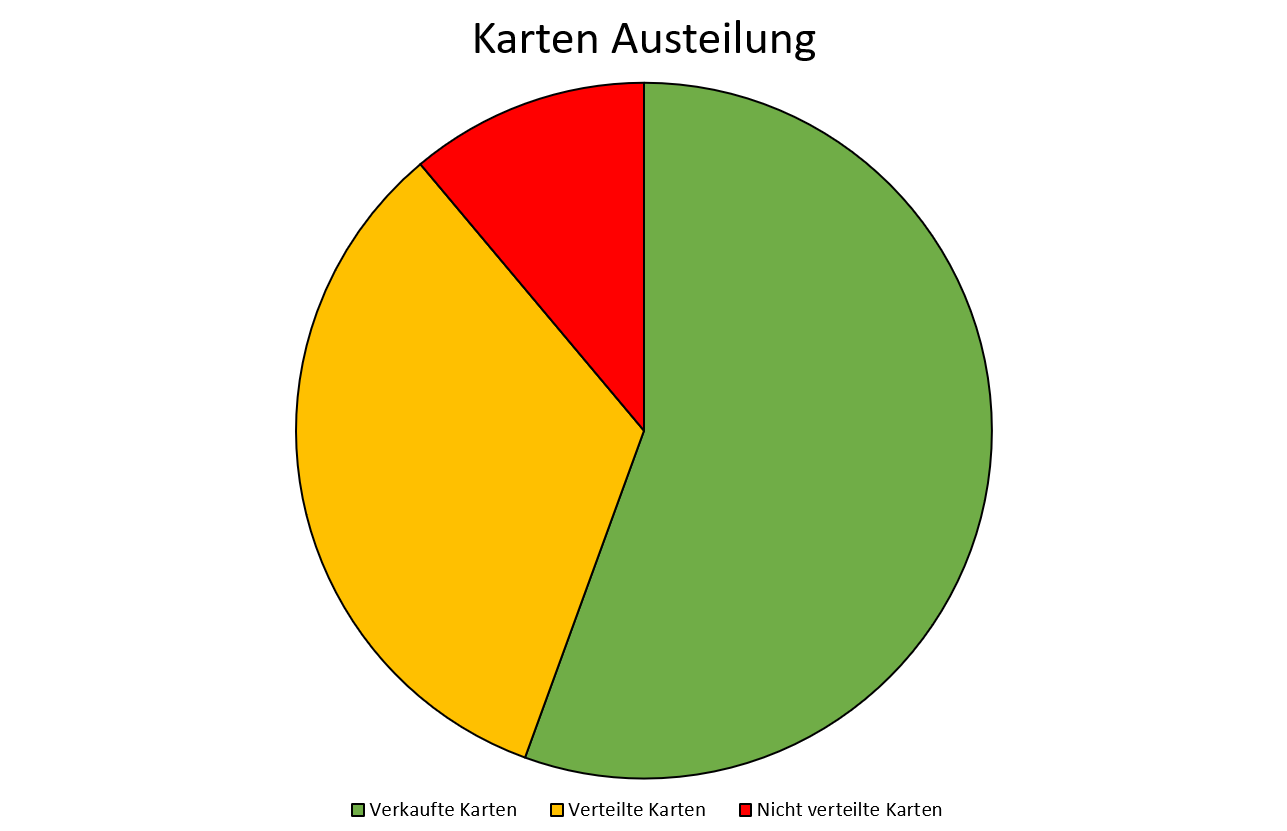
\includegraphics[width=\textwidth,height=\textwidth,keepaspectratio]{karten_austeilung.PNG}
					\caption{Verteilte Karten Diagram}
				\end{figure}

			\subsubsection{Eingetragene Kartenstände}
				Bei dieser Statistik handelt es sich um ein Balkendiagramm welches anzeigt wie oft die Promoter ihren Kartenstand eintragen. Dies hilft den Administratoren um zu sehen wie aktuell die Verkaufszahlen sind.
				
				\begin{figure}[H]
					\centering
					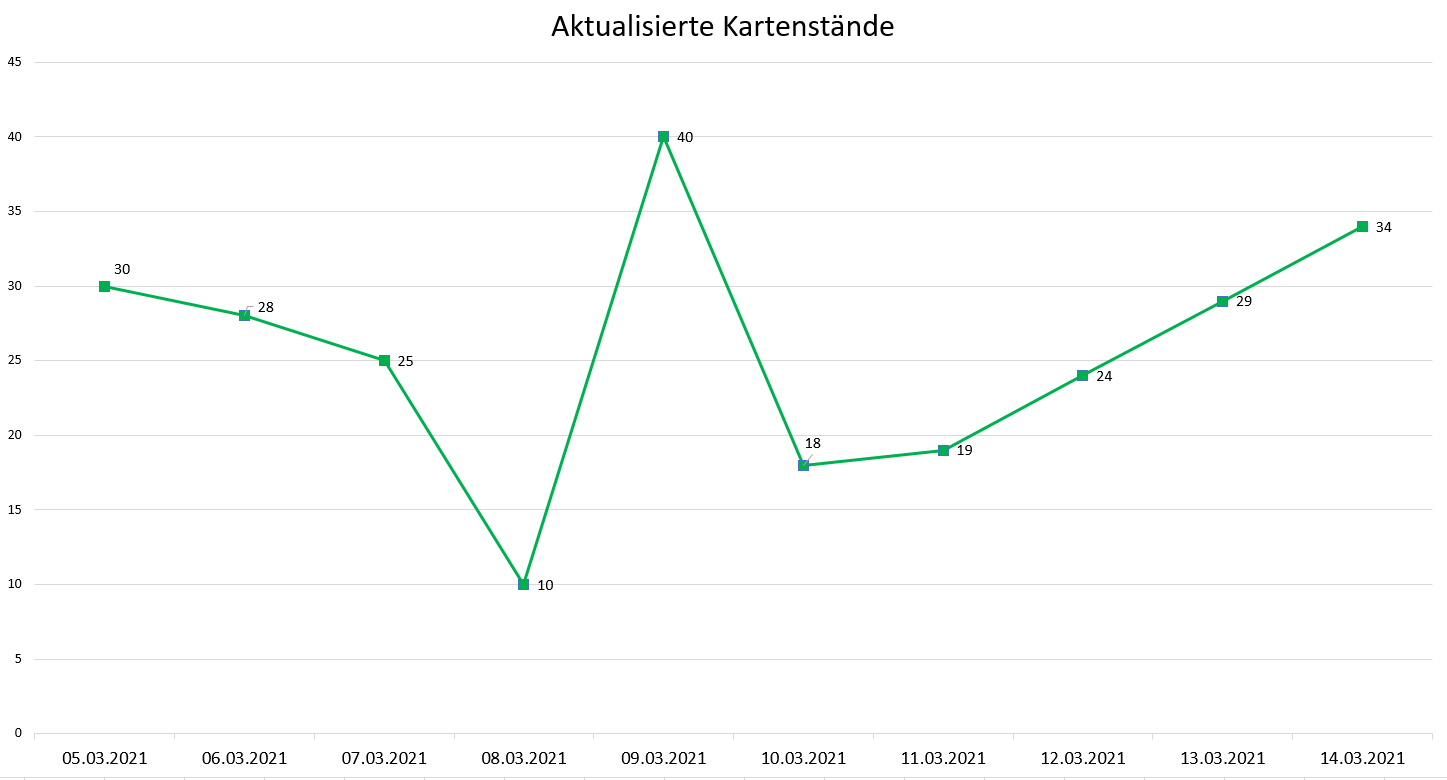
\includegraphics[width=\textwidth,height=\textwidth,keepaspectratio]{aktualisierte_kartenstaende.PNG}
					\caption{Eingetragene Kartenstände Diagram}
				\end{figure}

			\subsubsection{Verteilte Punkte}
				Die Statistik besteht aus einem Balkendiagramm welches zeigt wie viele Punkte bisher ausgegeben wurden und die Anzahl an Punkten welche bereits eingelöst wurden. Diese Statistik hilft den Administratoren zu sehen wie viele Punkte bisher verdient wurden und wie viele Punkte eingelöst wurden dies ermöglicht es abzuschätzen wie viele Goodies benötigt werden. 
				
				\begin{figure}[H]
					\centering
					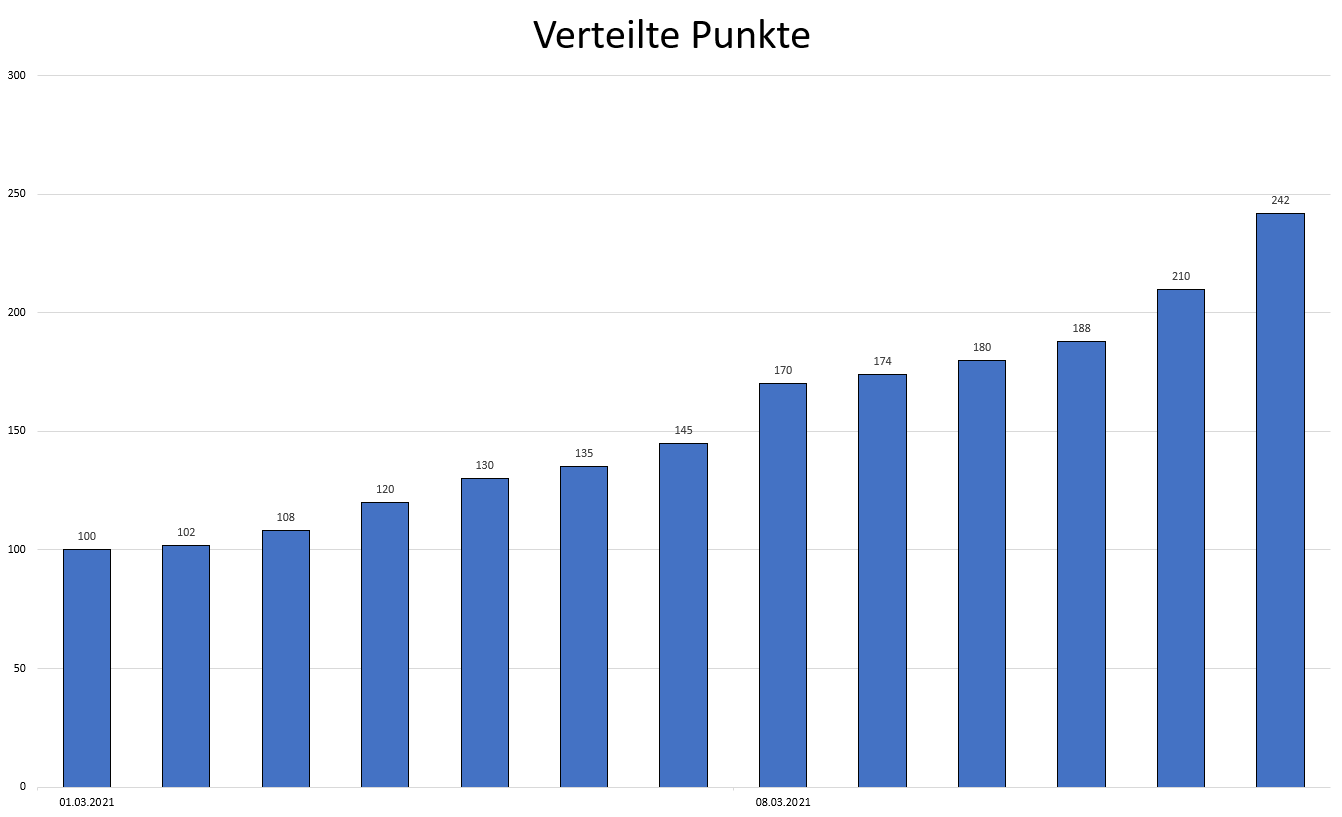
\includegraphics[width=\textwidth,height=\textwidth,keepaspectratio]{verteilte_punkte.PNG}
					\caption{Verteilte Karten Diagram}
				\end{figure}

			\subsubsection{Eingelösten Goodies}
				Diese Balkendiagramm zeigt an wie viel Goodies von einem Typen bisher eingelöst wurden. Dies hilft den Administratoren dabei die benötigten Goodies vorzubereiten und die Anzahl besser überwachen zu können. 

				\begin{figure}[H]
					\centering
					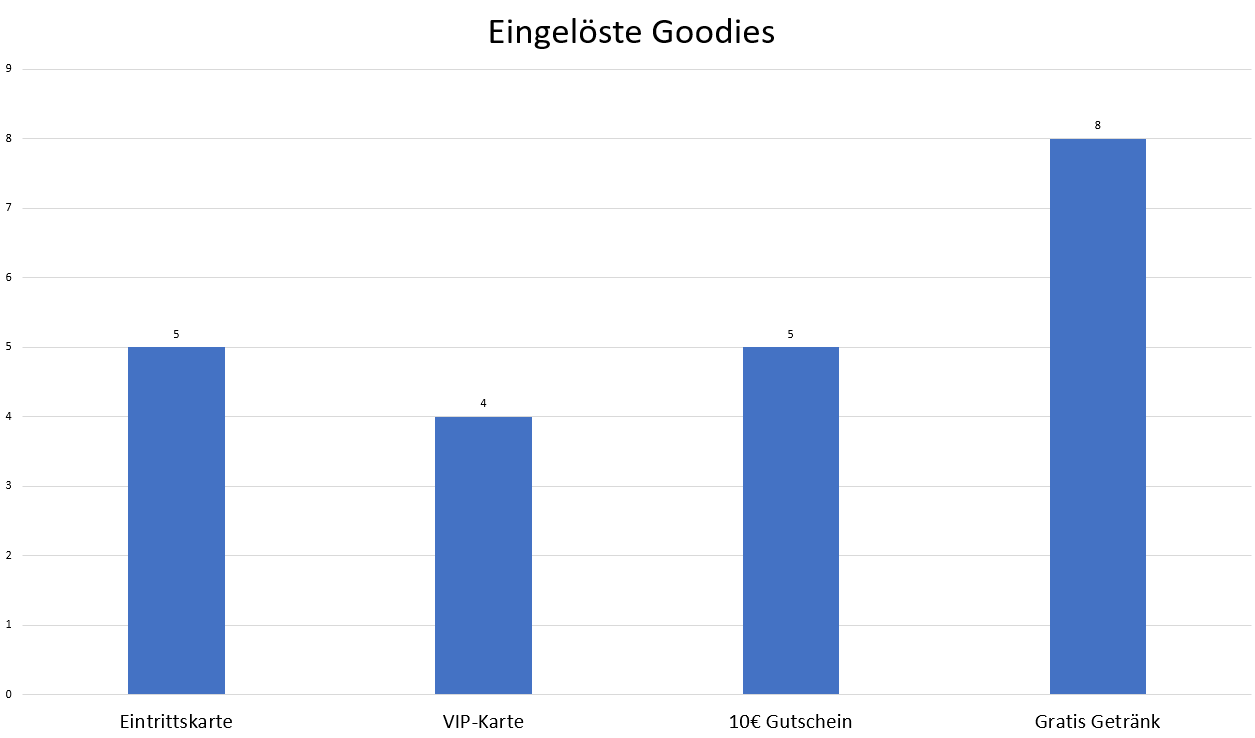
\includegraphics[width=\textwidth,height=\textwidth,keepaspectratio]{goodies.PNG}
					\caption{Eingelöste Goodies Diagram}
				\end{figure}
